In this chapter, we develop low-rank Gauss-Gauss detectors when observations from two
datasets are present. In such a setting, each dataset contains a target signal, which is
correlated with the other, that is assumed to reside in a low rank subspace. However, the
observations for each dataset are of high dimension and are corrupted with noise.  When
there is only one dataset present, this problem is referred to as matched subspace
detection. Matched subspace detectors are used in fields such as array processing
\cite{besson2006cfar, besson2005matched}, radar detection \cite{bandiera2007glrt,
  bandiera2007adaptive}, and handwriting recognition \cite{elden2007matrix}. The performance of matched
subspace detectors (MSDs) has been studied extensively when the signal subspace is known
\cite{mcwhorter2003matched, vincent2008matched, scharf1994matched, jin2005cfar} and
recently when the signal subspace is unknown \cite{asendorf2013performance,
  asendorf2012performance}. Here we explore the theory of MSDs when two multi-modal sets
of observations are available. Since these datasets both describe the same system, one
would hope that theoretically fusing feature vectors to account for correlations will
result in better detection ability. This chapter investigates using CCA to determine
whether these observations contain a target signal or whether they are pure noise.

We are motivated by the work in \cite{pezeshki2006canonical}, which shows that the
canonical basis is the right basis to use in low-rank detection. Here, Pezeshki, et
al., consider the signal plus noise model where an observation from one dataset is
available. This observation is a sum of a unknown low rank signal and Gaussian noise. They
apply CCA using the observation as the first modality and the unknown signal as the second
modality. We are interested in the different setting where we are presented with two
datasets, each possibly containing a low rank signal buried in high dimensional noise.

We begin by deriving a standard likelihood-ratio-test (LRT) given both observation
vectors. We then prove that this LRT may be written using the canonical vectors and
correlations returned by CCA. This demonstrates that the CCA basis is a correct basis to
use for Gauss-Gauss detection. We then discuss how to estimate unknown parameters in our
data model and provide empirical, plug-in detectors for both the LRT and CCA
detectors. Using numerical simulations, we demonstrate the extreme sub-optimality of the
empirical CCA detector compared to the plug-in LRT detector. Instead, using an ICCA
detector results in the same performance as the plug-in LRT detector, giving credence to
the previous idea that using only the informative components in data fusion is extremely
important. We provide a proof in the rank-1 setting that the plug-in and ICCA detectors
are equivalent.

\section{Data Model}

Formally, we are given two observation vectors,$y_1$ and $y_2$, of different modalities
(having different features). The goal is to design a detector to distinguish between the
$H_1$ hypothesis that the observations contain a target signal and the $H_0$ hypothesis
that the observations are purely noise. We model our observations by

\beq\label{eq:cca_detect_model} \ba &\text{Noise only, }&&H_0:\left\{ \ba
  & \yI = \xi_1 \\
  & \yII = \xi_2 \\
  \ea\right.\\
&\text{Signal plus noise, }&&H_1:\left\{ \ba
  & \yI = U_1\Sigma_1\,z_1 + \xi_1 \\
  & \yII = U_2\Sigma_2\,z_2 + \xi_2 \\
  \ea\right.\ea \eeq
where $U_1\in\complex^{d_1\times r_1}$ with mutually orthonormal columns,
$U_2\in\complex^{d_2\times r_2}$ with mutually orthonormal columns,
$\Sigma_1=\diag(\sigma_{11},\dots,\sigma_{1r_1})$,
$\Sigma_2=\diag(\sigma_{21},\dots,\sigma_{2r_2})$, with $\sigma_{1i},\sigma_{2i}>0$,
$\xi_1\sim\mathcal{N}(0,I_{d_1})$, $\xi_2\sim\mathcal{N}(0,I_{d_2})$, and 
\be
z=\left[\begin{array}{c}z_1
    \\z_2\end{array}\right]\sim\mathcal{N}\left(0,\left[\begin{array}{cc} I_{r_1} & P \\
      P^H & I_{r_2}\end{array}\right]\right),
\ee
 with $P\in\complex^{r_1\times r_2}$. Let $y=\left[\yI^H\,\yII^H\right]^H$ be the joint
 observation vector, $d=d_1+d_2$ be the dimension of $y$, and $r=r_1+r_2\ll d$ be the combined
 rank of the two low rank signal subspaces. 

\section{LRT Detector Derivation}
We consider the Neyman-Pearson setting for detection (see \cite{van1968detection}) where, given a
test observations from (\ref{eq:cca_detect_model}), we form $y$ as above by stacking the
individual observations in a column vector. The Neyman-Pearson lemma states that a
detector takes the form of a LRT
\beq\label{eq:lrt}
\Lambda(y) := \frac{f\left(y\,|\,H_1\right)}{f\left(y\,|\,H_0\right)}\detgtrless \gamma,
\eeq
where $\Lambda(y)$ is a test statistic, $\gamma$ is a threshold set to achieve a desired
false alarm rate, and $f$ is the appropriate conditional density of the observation.

The conditional distributions of $y$ under each hypothesis are
\be
\ba
& y|H_0 \sim\mathcal{N}(0,I_d) \\
& y|H_1 \sim\mathcal{N}(0,R_y),\\
\ea
\ee
where $R_y=\E{yy^H}$. Substituting these conditional distributions in (\ref{eq:lrt}) , the 
LRT statistic is
\be
\Lambda(y)=\frac{\mathcal{N}(0,R_y)}{\mathcal{N}(0,I_d)},
\ee
which can be simplified to
\beq\label{eq:lrt_stat}
\Lambda(y)=y^H\left(I_d-R_y^{-1}\right)y.
\eeq
The covariance matrix of the observation vector is
\be
\ba
&R_y &&=\left[\begin{array}{cc} \RI & \RIII \\ \RIII^H & \RII\end{array} \right] =
\left[\begin{array}{cc} 
U_1\Sigma_1\Sigma_1^HU_1^H + I_{d_1} &
U_1\Sigma_1P\Sigma_2^HU_2^H \\
U_2\Sigma_2P^H\Sigma_1^HU_1^H &
U_2\Sigma_2\Sigma_2^HU_2^H + I_{d_2} 
\end{array}\right]\\
&&& = \underbrace{\left[\begin{array}{cc}
U_1 & 0 \\ 0 & U_2
\end{array}\right]}_{U}
\underbrace{\left[\begin{array}{cc}
\Sigma_1 & 0 \\ 0 & \Sigma_2
\end{array}\right]}_{\Sigma}
\underbrace{\left[\begin{array}{cc}
    I_{r_1} & P \\ P^H & I_{r_2}
\end{array}\right]}_{R_z}
\underbrace{\left[\begin{array}{cc}
\Sigma_1^H & 0 \\ 0 & \Sigma_2^H
\end{array}\right]}_{\Sigma^H}
\underbrace{\left[\begin{array}{cc}
U_1^H & 0 \\ 0 & U_2^H
\end{array}\right]}_{U^H} + I_d\\
&&& = U\Sigma R_z\Sigma^HU^H + I_d. \\
\ea \ee 
Substituting this covariance matrix into the LRT statistic in (\ref{eq:lrt_stat}),
yields 
\be\ba
&\Lambda(y) &&=y^H\left(I_d-R_y^{-1}\right)y\\
&&& = y^H\left(I_d-\left(U\Sigma R_z\Sigma^HU^H+I_d\right)^{-1}\right)y\\
&&& = y^H\left(I_d-\left(I_d - U\left(\left(\Sigma R_z \Sigma^H\right)^{-1}+
    U^HU\right)\right)^{-1}U^H\right)y\\
&&& = y^H\left(I_d-\left(I_d - U\left(\Sigma^{-1} R_z^{-1} \Sigma^{-H}+I_r
    \right)^{-1}U^H\right)\right)y\\
&&& = y^HU\left(\Sigma^{-1} R_z^{-1} \Sigma^{-H}+I_r
\right)^{-1}U^Hy\\
&&& = y^HU\left(I_k -\Sigma^{-1}\left(R_z+ \Sigma^{-1}\Sigma^{-H}\right)^{-1}\Sigma^{-H}\right)U^Hy.\\
\ea\ee
The LRT detector is
\beq\label{eq:lrt_detect}
\Lambda_\text{lrt}(y) \detgtrless \gamma_{\text{lrt}}
\eeq
where $\Lambda_\text{lrt}(y)=y^HU\left(I_k -\Sigma^{-1}\left(R_z+
    \Sigma^{-1}\Sigma^{-H}\right)^{-1}\Sigma^{-H}\right)U^Hy$ and $\gamma_{\text{lrt}}$ is
a threshold set to satisfy $\Prob{\Lambda_{\text{lrt}}(y) > \gamma_{\text{lrt}}\,|\,H_0} =
\alpha$ where $\alpha$ is a desired false alarm rate. 

Writing the LRT statistic in this form is desirable for computational reasons. Instead of
inverting $R_y$, which is a $d\times d$ matrix of high dimension, we only need to invert
$\Sigma$ and $\left(R_z+ \Sigma^{-1}\Sigma^{-H}\right)$. Since $\Sigma$ is diagonal, its
inverse is easily computed. The second term is a $r\times r$ matrix, where $r\ll d$,
making it much easier to invert than $R_y$. If $y\in\reals^d$ then
\be
\Lambda_{\text{lrt}}(y)= y^HU\left(I_k -\Sigma^{-1}\left(R_z+ \Sigma^{-2}\right)^{-1}\Sigma^{-H}\right)U^Hy.
\ee

%\subsection*{Detectors based on $x$, $y$}
%We will also consider detectors based on the individual observations, $x$ and $y$. In a
%similar derivation, we can show that
%\be\ba
%&\Lambda(x) &&= \frac{\mathcal{N}(0,R_x)}{\mathcal{N}(0,I_p)} = x^H(I_p-R_{xx})x\\
%&&& = x^H\left(U_x\left(\Sigma_x^{-2}+I_{k_x}\right)^{-1}\right)x\\
%&&& = x^HU_x\tilde{\Sigma}_xU_x^Hx\\
%\ea\ee
%where $\tilde{\Sigma}_x=\diag\left(\frac{\sigma_{xi}^2}{\sigma_{xi}^2+1}\right)$.

%Similarly,
%\be
%\Lambda(y) = y^HU_y\tilde{\Sigma}_yU_y^Hy
%\ee
%with $\tilde{\Sigma}_y=\diag\left(\frac{\sigma_{yi}^2}{\sigma_{yi}^2+1}\right)$.

\section{CCA Detector Equivalency}
In this section, we will show that the LRT derived above in (\ref{eq:lrt_detect}) can be
written using the canonical vectors and correlation coefficients found by CCA.

Recall that the matrix of interest in CCA is $C=\RI^{-1/2}\RIII\RII^{-1/2}$ and that the
canonical vectors and correlation coefficients are found by solving the SVD of
$C=FKG^H$. We begin by manipulating the covariance matrix of $y$.

\be\ba
&R_y &&= \left[\begin{array}{cc}
    \RI & \RIII \\ \RIII^H & \RII
\end{array}\right] = 
\left[\begin{array}{cc}
    \RI^{1/2} & 0 \\ 0 & \RII^{1/2}
\end{array}\right]\left[\begin{array}{cc}
  I_{d_1} & C \\ C^H & I_{d_2}
\end{array}\right]\left[\begin{array}{cc}
  \RI^{H/2} & 0 \\ 0 & \RII^{H/2}
\end{array}\right]\\
&&& = \left[\begin{array}{cc}
    \RI^{1/2} & 0 \\ 0 & \RII^{1/2}
\end{array}\right]\left[\begin{array}{cc}
    F & 0\\ 0 & G
\end{array}\right]\left[\begin{array}{cc}
  I_{d_1} & K \\ K^H & I_{d_2}
\end{array}\right]\left[\begin{array}{cc}
    F^H & 0 \\ 0 & G^H
\end{array}\right]\left[\begin{array}{cc}
   \RI^{H/2} & 0 \\ 0 & \RII^{H/2}
\end{array}\right].\\
\ea\ee
Using this decomposition, the inverse of the covariance matrix of $y$ is
\be
R_y^{-1} = \left[\begin{array}{cc}
    \RI^{-1/2} & 0 \\ 0 & \RII^{-1/2}
\end{array}\right]\left[\begin{array}{cc}
    F & 0\\ 0 & G
\end{array}\right]\left[\begin{array}{cc}
    I_{d_1} & K \\ K^H & I_{d_2}
\end{array}\right]^{-1}\left[\begin{array}{cc}
    F^H & 0 \\ 0 & G^H
\end{array}\right]\left[\begin{array}{cc}
    \RI^{-H/2} & 0 \\ 0 & \RII^{-H/2}
\end{array}\right].\\
\ee Recall that the $i$-th canonical vectors returned by CCA are
\be\ba
& \xI^{(i)} = \RI^{-1/2}f_i\\
& \xII^{(i)} = \RII^{-1/2}g_i\\
\ea\ee
 where $f_i$ and $g_i$ are the left and right singular vectors of $C$ corresponding
to the $i$-th largest singular value, $k_i$, respectively. Define the matrices 
\be\ba
&X_1 =\left[\xI^{(1)},\dots, \xI^{(d_1)}\right]= \RI^{-1/2}F
&X_2=\left[\xII^{(1)},\dots,\xII^{(d_2)}\right] = \RII^{-1/2}G
\ea\ee
 to be the matrices of canonical vectors
returned by CCA. Using this notation and substituting the expression for $R_y^{-1}$ in the
LRT statistic in (\ref{eq:lrt_stat}), we arrive at 
\be\ba
&\Lambda(y)&&= y^H\left(I_d -R_y^{-1}\right)y\\
&&&=y^H\left(I_d - \left[\begin{array}{cc} X_1 & 0 \\ 0 & X_2
\end{array}\right]\left[\begin{array}{cc}
    I_{d_1} & K \\ K^H & I_{d_2}
\end{array}\right]^{-1}\left[\begin{array}{cc}
  X_1^H & 0 \\ 0 & X_2^H
\end{array}\right]\right)y.\\
\ea\ee 
The above expression is written in terms of the observation $y$, the canonical
vectors $X_1$ and $X_2$ and the correlation coefficients $K$ returned by CCA. This
statistic is exactly equivalent to the LRT statistic derived earlier. Therefore, we
conclude that the CCA basis is the correct basis to use in such low-rank Gauss-Gauss
detection with two datasets.

We can write this detector slightly differently by recalling that the
canonical variates are $w_1^{(i)}=x_1^{(i)H}y$ and $w_2^{(i)}=x_2^{(i)H}y$. Let
$w_1=\left[w_1^{(1)},\dots,w_1^{(d_1)}\right]^H$,
$w_2=\left[w_2^{(1)},\dots,w_2^{(d_2)}\right]^H$, and define
\be 
w = \left[\begin{array}{c}\wI \\ \wII\end{array}\right] =
\left[\begin{array}{cc}X_1^H & 0 \\ 0 & X_2^H\end{array}\right]y. 
\ee
Using this definition and defining
\be
X = \left[\begin{array}{cc}X_1 & 0 \\ 0 & X_2\end{array}\right],
\ee
the above detector may be written
\beq\label{eq:cca_stat}
\Lambda_{\text{cca}}(w) = w^H\left(\left(X^HX\right)^{-1}-\left[\begin{array}{cc}
    I_{d_1} & K \\ K^H & I_{d_2}
\end{array}\right]^{-1}\right)w.
\eeq
In conclusion, we have derived a general CCA detector that takes the canonical variates as
inputs and uses only the canonical vectors $X$ and the canonical correlation coefficients
$K$ in its statistic. This detector is
\beq\label{eq:cca_detect}
\Lambda_{\text{cca}}\detgtrless\gamma_{\text{cca}}
\eeq
where $\Lambda_{\text{cca}}(w)$ is defined in (\ref{eq:cca_stat}) and
$\gamma_{\text{cca}}$ is a threshold set to satisfy\\
$\Prob{\Lambda_{\text{cca}}(w)>\gamma_{\text{cca}}\,|\,H_0}=\alpha$ where $\alpha$ is the
desired false alarm rate. The CCA detector in (\ref{eq:cca_detect}) is equivalent to the
LRT detector in (\ref{eq:lrt_detect}). This is a general proof and is independent of the
data models placed on $y$. That is, in this proof, we did not refer to the data model in
(\ref{eq:cca_detect_model}) that motivated the problem.

\subsection{CCA Detector for Data Model (\ref{eq:cca_detect_model})}
The above CCA detector was derived for a generic data model. Here we find the canonical
vectors and correlation coefficients for the data model described in
(\ref{eq:cca_detect_model}). Under this model, the data covariance matrices are
\be\ba
&\RI = U_1\Sigma_1\Sigma_1^HU_1^H + I_{d_1}\\
&\RII = U_2\Sigma_2\Sigma_2^HU_2^H + I_{d_2}\\
&\RIII = U_1\Sigma_1P\Sigma_2^HU_2^H\\
\ea\ee
and their inverses are
\be\ba
&\RI^{-1} = \left[\begin{array}{cc}U_1 & U_1^\perp\end{array}\right]
\left[\begin{array}{cc}\left(\Sigma_1\Sigma_1^H + I_{r_1}\right)^{-1} & 0 \\ 0 &
    I_{d_1-r_1} \end{array}\right]  \left[\begin{array}{c} U_1^H \\ U_1^{H\perp} 
  \end{array}\right] \\
&\RI^{-1} = \left[\begin{array}{cc}U_2 & U_2^\perp\end{array}\right]
\left[\begin{array}{cc}\left(\Sigma_2\Sigma_2^H + I_{r_2}\right)^{-1} & 0 \\ 0 &
    I_{d_2-r_2} \end{array}\right]  \left[\begin{array}{c} U_2^H \\ U_2^{H\perp} 
  \end{array}\right]. \\
\ea\ee 
It follows that the CCA matrix $C$ is 
\beq\label{eq:cca_detec_C}\ba
& C &&= \RI^{-1/2}\RIII\RII^{-1/2}\\
&&& = U_1\left(\Sigma_1\Sigma_1^H +I_{r_1}\right)^{-1/2}\Sigma_1 R_z \Sigma_2\left(\Sigma_2\Sigma_2^H+I_{r_2}\right)^{-1/2}U_2^H.\\
\ea\eeq Clearly, when expressed in (\ref{eq:cca_detec_C}), $C$ is a $\min\left(r_1,r_2\right)$ rank
matrix. This implies that there are only $r^*:=\min\left(r_1,r_2\right)$ non-zero correlation
coefficients. Therefore, there are only $r^*$ canonical vectors that should be used in a
detector. Define \be\ba
&X_{1,r^*} = X_1(:,1:r^*)\\
&X_{2,r^*} = X_2(:,1:r^*)\\
&K_{r^*} = K(1:r^*,1:r^*)\\
\ea\ee as the trimmed canonical vectors and correlation coefficients. Finally define 
\be
X_{r^*} = \left[\begin{array}{cc}X_{1,r^*} &0 \\ 0 & X_{2,r^*}\end{array}\right] 
\ee and
$w_{r^*} = X_{r^*}^Hy$. Then the CCA detector is 
\beq\label{eq:cca_stat_r}
\Lambda_{\text{cca}}(w_{r^*}) =
w_{r^*}^H\left(\left(X_{r^*}^HX_{r^*}\right)^{-1}-\left[\begin{array}{cc} I_{r^*} &
      K_{r^*} \\ K_{r^*}^H & I_{r^*} \end{array}\right]^{-1}\right)w_{r^*},
\eeq
which only uses the $r^*$ nonzero CCA correlation coefficients and corresponding 
canonical vectors.

\section{Empirical Detectors}

In many applications, the target signal matrices $U_1$,$U_2$, their SNR matrices
$\Sigma_1$,$\Sigma_2$, and the correlation matrix between datasets $R_z$ are unknown and
thus the resulting data covariance matrices are unknown. Therefore, neither the LRT
statistic in (\ref{eq:lrt_detect}) or the CCA statistic in (\ref{eq:cca_stat_r}), which
relies on $C$ in (\ref{eq:cca_detec_C}) can be computed. In such settings, we are given
training data to estimate any unknown parameters. This section will describe how to
estimate these unknown parameters and use these estimates in the previously derived
detectors. We then will describe how to use ICCA for detection and show its equivalence to
the plug-in LRT detector. Finally, we close with numerical simulations demonstrating that
the ICCA detector achieves the same performance as the plug-in LRT and that the
empirical CCA detector is extremely suboptimal.

\subsection{Parameter Estimation}\label{sec:param_estims}

Assume that we are given $n$ observations of each dataset, $\yI^{(1)},\dots,
\yI^{(n)}$, and $\yII^{(1)},\dots, \yII^{(n)}$. We stack these observations into two
training data matrices $Y_1=\left[\yI^{(1)},\dots, \yI^{(n)}\right]$, and
$Y_2=\left[\yII^{(1)},\dots, \yII^{(n)}\right]$. We assume that $r_1$ and $r_2$ are
known. Let $Q_1D_1V_1^H$ be the SVD of $\frac{1}{\sqrt{n}}Y_1$ and let $Q_2D_2V_2^H$ be
the SVD of $\frac{1}{\sqrt{n}}Y_2$. The ML estimates of our unknown parameters are 

\be\ba
&\widehat{U}_1 = Q_x(:,1:r_1),\,\,\,\widehat{U}_2 = Q_2(:,1:r_2),\,\,\,
\widehat{U}=\left[\begin{array}{cc}\widehat{U}_1 & 0 \\ 0 &
    \widehat{U}_2\end{array}\right]\\
&\widehat{\Sigma}_1 = \left(D_1^2(1:r_1,1:r_1)-I_{r_1}\right)^{1/2},\,\,\, 
\widehat{\Sigma}_2 = \left(D_2^2(1:r_2,1:r_2)-I_{r_2}\right)^{1/2},\,\,\,
\widehat{\Sigma}=\left[\begin{array}{cc}\widehat{\Sigma}_1 & 0 \\ 0 &
    \widehat{\Sigma}_2\end{array}\right]\\
&\RIhat = Q_1D_1D_1^HQ_1^H,\,\,\,
\RIIhat= Q_2D_2D_2^HQ_2^H,\,\,\,
\RIIIhat = Q_1D_1V_1^HV_2D_2^HU_2^H\\
&\widehat{P}=\widehat{\Sigma}_1^{-1}\widehat{U}_1^H\RIIIhat
\widehat{U}_2\widehat{\Sigma}_2^{-1} = \widehat{\Sigma}_1^{-1}D_1(1:r_1,:)
V_1^HV_2D_2(1:r_2,:)^H\widehat{\Sigma}_2^{-1}.\\ 
\ea\ee

\subsection{Rank-1 Detectors}

We consider the most simple setting, when $r_1=r_2=1$ so that $P$ is simply a scalar,
which we will denote $\rho$. In this setting, the parameter estimates simplify to 
\be\ba &
\widehat{U}=\left[\begin{array}{cc}Q_1(:,1) & 0 \\ 0 &
    Q_2(:,1)\end{array}\right]\\
& \widehat{\Sigma}=\left[\begin{array}{cc}\sqrt{d_{11}^2-1} & 0 \\ 0 &
    \sqrt{d_{21}^2 -1}\end{array}\right]\\
& \widehat{P}=\widehat{\rho}=\frac{d_{11}d_{21}V_1(:,1)^HV_2(:,1)}{\sqrt{d_{11}^2
    -1}\sqrt{d_{21}^2-1}} \\
& \widehat{R}_z = \left[\begin{array}{cc}1 &\widehat{\rho}\\ \widehat{\rho} &
    1\end{array}\right]
\ea\ee
where $d_{11}$ is the largest singular value of $Y_1$ and $d_{21}$ is the largest singular
value of $Y_2$. 

To form a realizable LRT detector, we plug in these estimates into the statistic in
(\ref{eq:lrt_stat}). This results in the plug-in LRT statistic
\beq\label{eq:plugin_lrt_stat}
\Lambda_\text{plugin}(y)=y^H\widehat{U}\left(I_2 -\widehat{\Sigma}^{-1}\left(\widehat{R}_z+
    \widehat{\Sigma}^{-1}\widehat{\Sigma}^{-H}\right)^{-1}\widehat{\Sigma}^{-H}\right)
\widehat{U}^Hy.
\eeq

Similarly, we create a realizable CCA detector by performing empirical CCA as described in
Section \ref{sec:emp_cca} by forming 
\be
\widehat{C} =\RIhat^{-1/2}\RIIIhat\RIIhat^{-1/2}=Q_1I_{d_1\times n}V_1^HV_2 I_{n\times
  d_2} Q_2^H.
\ee
We then use the largest (as $r^*=1$) singular value and corresponding left and right
singular vectors of $\widehat{C}$ to form estimates of the canonical vectors and
correlation coefficient. Specifically, let $\widehat{f}_1$ and $\widehat{g}_1$ be the
left and right singular vectors corresponding to the largest singular value
$\widehat{k}_1$. Then the estimates of the canonical vectors and correlation coefficient
are
\beq\label{eq:emp_cca_detec_params}\ba
& \widehat{K}_{r^*} = \widehat{k}_1\\
&\widehat{X}_{r^*} = \left[\begin{array}{cc}\RIhat^{-1/2}\widehat{f}_1 & 0 \\ 0 &
    \RIIhat^{-1/2}\widehat{g}_1\end{array}\right]\\
& \widehat{w}_{r^*} = \widehat{X}_{r^*}^H y.\\
\ea\eeq
We then substitute these estimates into the CCA detector in (\ref{eq:cca_stat_r}).
This results in the empirical CCA detector statistic 
\beq\label{eq:cca_plugin_stat}
\Lambda_{\text{cca}}(\widehat{w}_{r^*}) =
\widehat{w}_{r^*}^H\left(\left(\widehat{X}_{r^*}^H\widehat{X}_{r^*}\right)^{-1} -
  \left[\begin{array}{cc} 1 & \widehat{k}_1 \\ \widehat{k}_1 & 1 \end{array}\right]^{-1}
\right)\widehat{w}_{r^*}.  
\eeq 
However, we saw in Chapter \ref{sec:cca} that empirical
CCA is suboptimal and that we can avoid some of the performance loss of CCA by
informatively trimming data components before computing the canonical vectors. We apply
that principle here to form an ICCA detector. We instead take the top singular value,
$\widetilde{k}_1$ and corresponding singular vectors $\widetilde{f}_1$ and
$\widetilde{g}_1$ of the matrix $\widetilde{C} =
Q_1(:,1)V_1(:,1)^HV_2(:,1)U_2(:,1)^H$. Using this rank-1 SVD, we form informative
canonical vectors and correlation coefficient similarly as in
(\ref{eq:emp_cca_detec_params}). Substituting these informative parameters into the CCA
detector in (\ref{eq:cca_stat_r}) results in the ICCA detector statistic  
\beq\label{eq:icca_plugin_stat} \Lambda_{\text{icca}}(\widetilde{w}_{r^*}) =
\widetilde{w}_{r^*}^H\left(\left(\widetilde{X}_{r^*}^H\widetilde{X}_{r^*}\right)^{-1} -
  \left[\begin{array}{cc} 1 & \widetilde{k}_1 \\ \widetilde{k}_1 & 1 \end{array}\right]^{-1}
\right)\widetilde{w}_{r^*}.  
\eeq

\subsection{Rank 1 Proof that $\Lambda_{\text{icca}}(\widetilde{w}_{r^*})
  \equiv\Lambda_{\text{plug-in}}(y)$}

In this section, we prove that the ICCA detector statistic in (\ref{eq:icca_plugin_stat})
is equivalent to the plug-in LRT statistic in (\ref{eq:plugin_lrt_stat}) when $r^*=r_1=r_2=1$. 
Recall that we are interested in the largest singular value and corresponding singular
vectors of the matrix $\widetilde{C} = Q_1(:,1)V_1(:,1)^HV_2(:,1)U_2(:,1)^H$ used in
ICCA. In the rank-1 setting, $\widetilde{C}$ is a rank-1 matrix, and we immediately
see that $\widetilde{f}_1=Q_1(:,1)$, $\widetilde{g}_1=Q_2(:,1)$, and
$\widetilde{k}_1=V_1(:,1)^HV_2(:,1)$. Therefore, the canonical vectors are
\be\ba
&\widetilde{X}_{r^*} &&= \left[\begin{array}{cc}\RIhat^{-1/2}\widetilde{f}_1 & 0 \\ 0 &
    \RIIhat^{-1/2}\widetilde{g}_1 \end{array}\right]\\
&&& = \left[\begin{array}{cc}\widehat{U}_1\left(\widehat{\Sigma}_1\widehat{\Sigma}_1^H +
      1\right)^{-1/2}  & 0 \\ 0 &
    \widehat{U}_2\left(\widehat{\Sigma}_2\widehat{\Sigma}_2^H  +
      1\right)^{-1/2}\end{array}\right]\\ 
&&& = \widehat{U}\left(\widehat{\Sigma}\widehat{\Sigma}^H + I_{2}\right)^{-1/2}\\
\ea\ee
and the canonical variates are $\widetilde{w}_{r^*} = \widetilde{X}_{r^*}^Hy =
\left(\widehat{\Sigma}\widehat{\Sigma}^H + I_{2}\right)^{-1/2}\widehat{U}^Hy$. Therefore,
we can write the ICCA detector as

\be\ba &\Lambda_{\text{icca}}(\widetilde{w}_{r^*}) &&=
\widetilde{w}_{r^*}^H\left(\left(\widetilde{X}_{r^*}^H\widetilde{X}_{r^*}\right)^{-1} -
  \left[\begin{array}{cc} 1 & \widetilde{k}_1 \\ \widetilde{k}_1 &
      1 \end{array}\right]^{-1}
\right)\widetilde{w}_{r^*}\\
&&& = y^H\widehat{U}\left(\widehat{\Sigma}\widehat{\Sigma}^H + I_{2}\right)^{-1/2}\left(
  \left(\widehat{\Sigma}\widehat{\Sigma}^H + I_2\right) - \left[\begin{array}{cc} 1 &
      \widetilde{k}_1 \\ \widetilde{k}_1 & 1 \end{array}\right]^{-1}
\right)\left(\widehat{\Sigma}\widehat{\Sigma}^H + I_{2}\right)^{-1/2}\widehat{U}^Hy\\
&&& = y^H\widehat{U}\left(I_2 - \left(\widehat{\Sigma}\widehat{\Sigma}^H +
    I_{2}\right)^{-1/2} \left[\begin{array}{cc} 1 & \widetilde{k}_1 \\ \widetilde{k}_1 &
      1 \end{array}\right]^{-1}\left(\widehat{\Sigma}\widehat{\Sigma}^H +
    I_{2}\right)^{-1/2}\right)\widehat{U}^Hy\\
&&& = y^H\widehat{U}\left(I_2 - \left[\begin{array}{cc}
      \widehat{\Sigma}_1\widehat{\Sigma}_1^H + 1 &
      d_{11}\widetilde{k}_1d_{21} \\
      d_{21}\widetilde{k}_1d_{11} & \widehat{\Sigma}_2\widehat{\Sigma}_2^H
      +1 \end{array}\right]^{-1}\right)\widehat{U}^Hy\\
&&& = y^H\widehat{U}\left(I_2 - \left[\begin{array}{cc}
      \widehat{\Sigma}_1\widehat{\Sigma}_1^H + 1 & d_{11}V_1(:,1)^HV_2(:,1)d_{21} \\
      d_{21}V_2(:,1)^HV_1(:,1)d_{11} & \widehat{\Sigma}_2\widehat{\Sigma}_2^H
      +1 \end{array}\right]^{-1}\right)\widehat{U}^Hy\\
&&& = y^H\widehat{U}\left(I_2 - \left(\widehat{\Sigma}\left[\begin{array}{cc} 1 &
        \widehat{P} \\ \widehat{P}^H &
        1  \end{array}\right]\widehat{\Sigma}^H+I_2\right)^{-1}\right)\widehat{U}^Hy\\
&&& = y^H\widehat{U}\left(I_2 - \left(\widehat{\Sigma}\widehat{R}_z
    \widehat{\Sigma}^H+I_2\right)^{-1}\right)\widehat{U}^Hy\\
&&& = y^H\widehat{U}\left(I_2 - \widehat{\Sigma}^{-1}\left(\widehat{R}_z +
    \widehat{\Sigma}^{-1}\widehat{\Sigma}^{-H}\right)^{-1}\widehat{\Sigma}^{-1}
\right)\widehat{U}^Hy.\\
\ea\ee

This is exactly the expression for the plug-in LRT statistic.

\subsection{Rank 1 Numerical Simulations}

We now use numerical simulations to explore the performance of the plug-in LRT detector in
(\ref{eq:plugin_lrt_stat}), the empirical CCA detector in (\ref{eq:icca_plugin_stat}), and
the ICCA detector in (\ref{eq:cca_plugin_stat}) in the rank-1 setting where
$r_1=r_2=1$. Specifically, we wish to show that the plug-in LRT detector is
equivalent to the ICCA detector. We also wish to explore how the performance of the
CCA detector in compares to that of the plug-in LRT detector, because in theory these
detectors are equivalent.

To compare the performance of these detectors, we compute empirical ROC curves. To
compute an empirical ROC curve, we first generate  two random signal vectors, $u_1$ and
$u_2$, by taking the first left singular vector of two appropriately sized random
matrices with i.i.d. $\mathcal{N}(0,1)$ entries. In this simulation we make the
simplifying assumption that $\sigma_1=\sigma_2$. Given a desired SNR, correlation $\rho$,
and random $u_1$ and $u_2$, we generate $n$ training samples of $\yI$ and $\yII$ from the
$H_1$ hypothesis in (\ref{eq:cca_detect_model}). Using these training samples, we form
estimates $\widehat{U}$, $\widehat{\Sigma}$, $\widehat{\rho}$, $\RIhat$, $\RIIhat$, and
$\RIIIhat$ as described in Section \ref{sec:param_estims}.

We then generate a desired number of test samples from each hypothesis using
(\ref{eq:cca_detect_model}). For each test sample, we compute the test statistic for the
plug-in LRT, empirical CCA, and ICCA detectors in (\ref{eq:plugin_lrt_stat}),
(\ref{eq:cca_plugin_stat}), and (\ref{eq:icca_plugin_stat}), respectively. Using Fawcett's
\cite{fawcett2006introduction} `Algorithm 2', we compute an empirical ROC curve by first
sorting the test statistics for a given detector. At each statistic, we log a ($P_F$,
$P_D$) pair by counting the number of lower scores generated from each hypothesis. This is
repeated for multiple realizations of $u_1$ and $u_2$, generating multiple empirical ROC
curves for each detector. We refer to a single empirical ROC curve corresponding to a
realization of $u_1$ and $u_2$ as a trial. We then average the empirical ROC curves for a
detector over multiple trials using Fawcett's \cite{fawcett2006introduction} `Algorithm
4'. This performs threshold averaging by first uniformly sampling the sorted list of all
test scores of ROC curves and then computing ($P_F$, $P_D$) pairs in the same way as
`Algorithm 2'.

To compare the ROC curves of different detectors, we use the area under the ROC curve
(AUC) statistic. The AUC statistic ranges between 0.5, which represents a random guessing
detector, and 1.0, which represents a detector that can perfectly distinguish between the
two hypotheses. We compute the ROC curves and their respective AUC for many values of the
number of training samples, $n$, and SNR $\sigma=\sigma_1=\sigma_2$. We present the AUC
results in the form of a heatmap for two different values of $\rho$ for each of the
detectors. Figure \ref{fig:auc_high_rho} presents results for $\rho=0.8$ and Figure
\ref{fig:auc_low_rho} presents results for $\rho = 0.2$.

\begin{figure} 
  \subfigure[Plug-in LRT]{
    \centering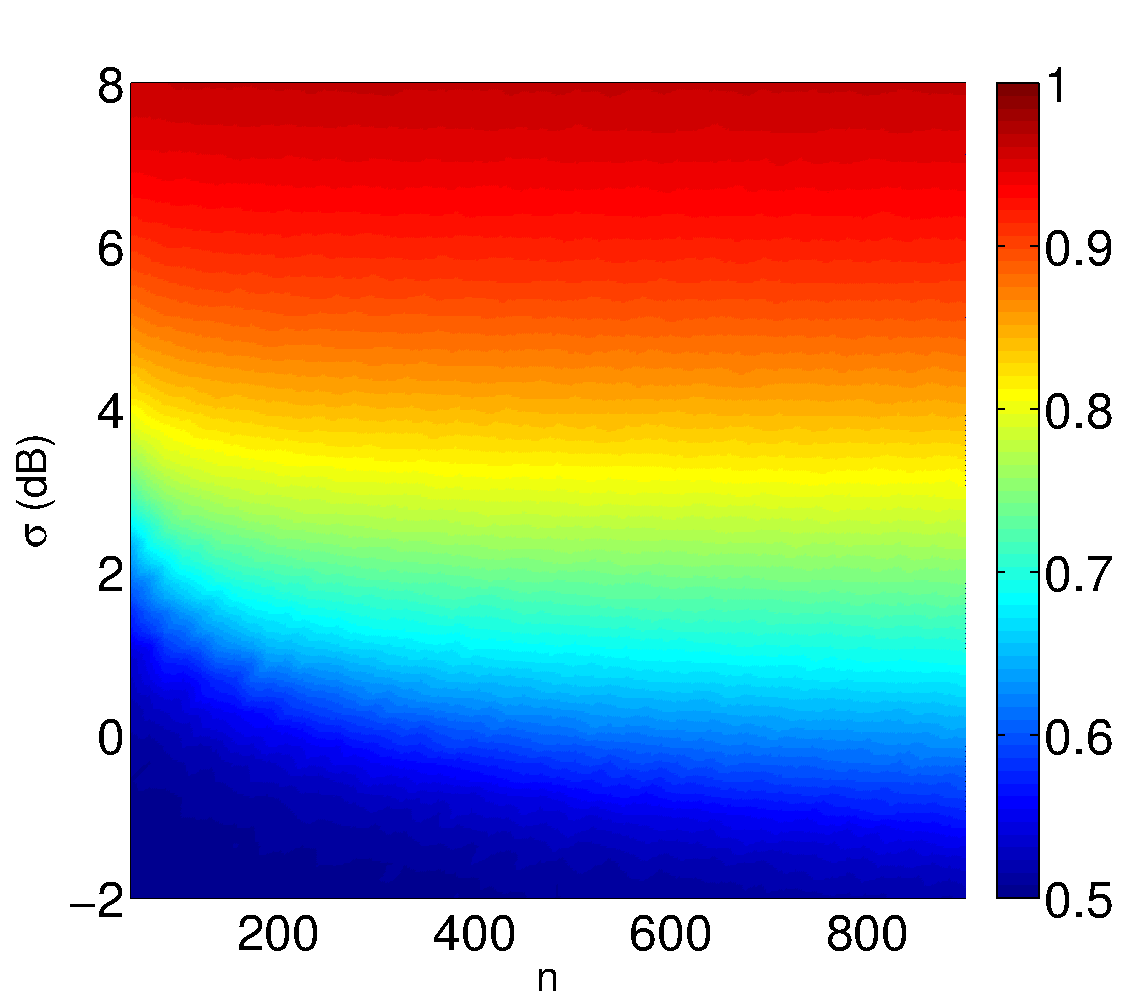
\includegraphics[width=\figwidth]{figures/auc_lrt_high_rho.pdf}
    \label{fig:auc_lrt_high_rho}
  }
  \subfigure[ICCA]{
    \centering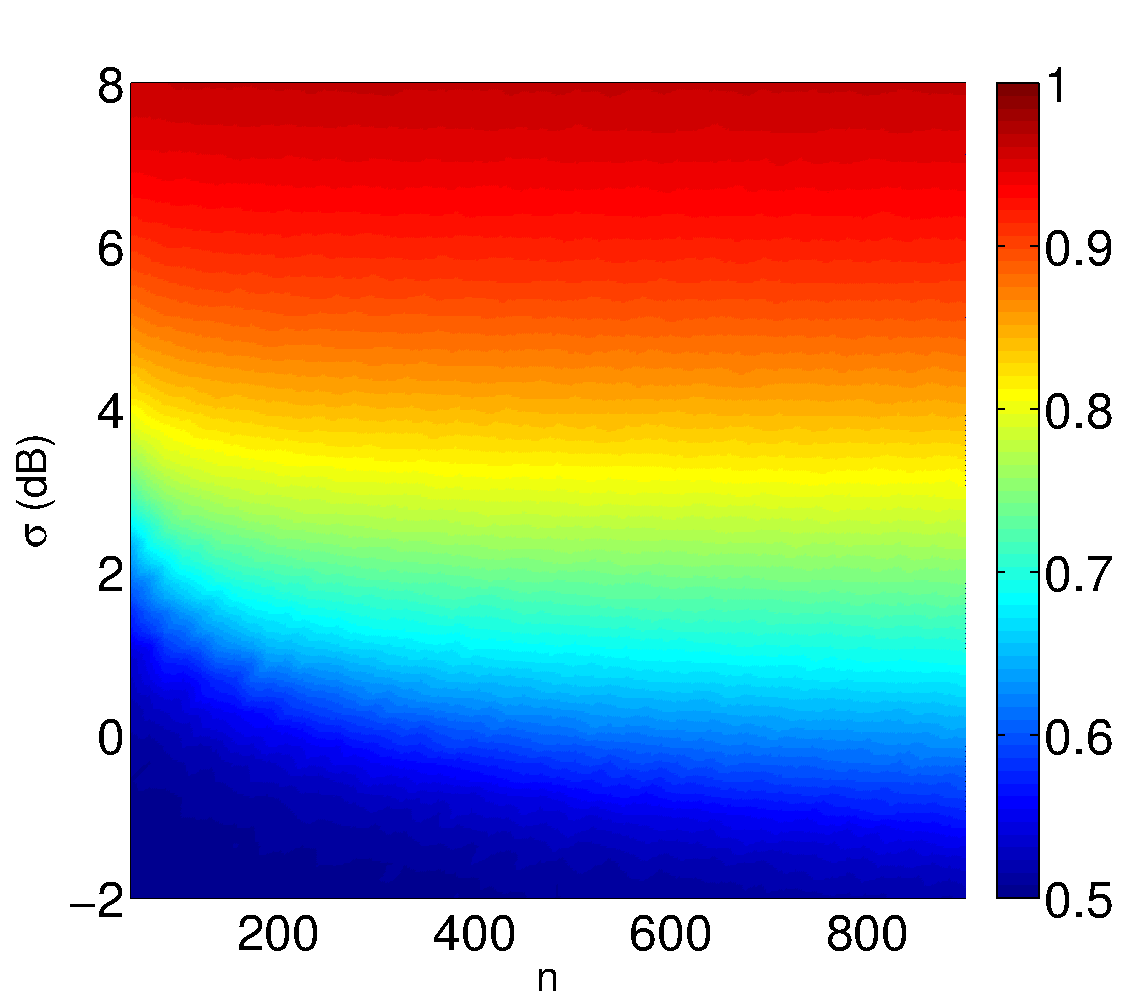
\includegraphics[width=\figwidth]{figures/auc_icca_high_rho.pdf}
    \label{fig:auc_icca_high_rho}
  }
  \subfigure[Empirical CCA]{
    \centering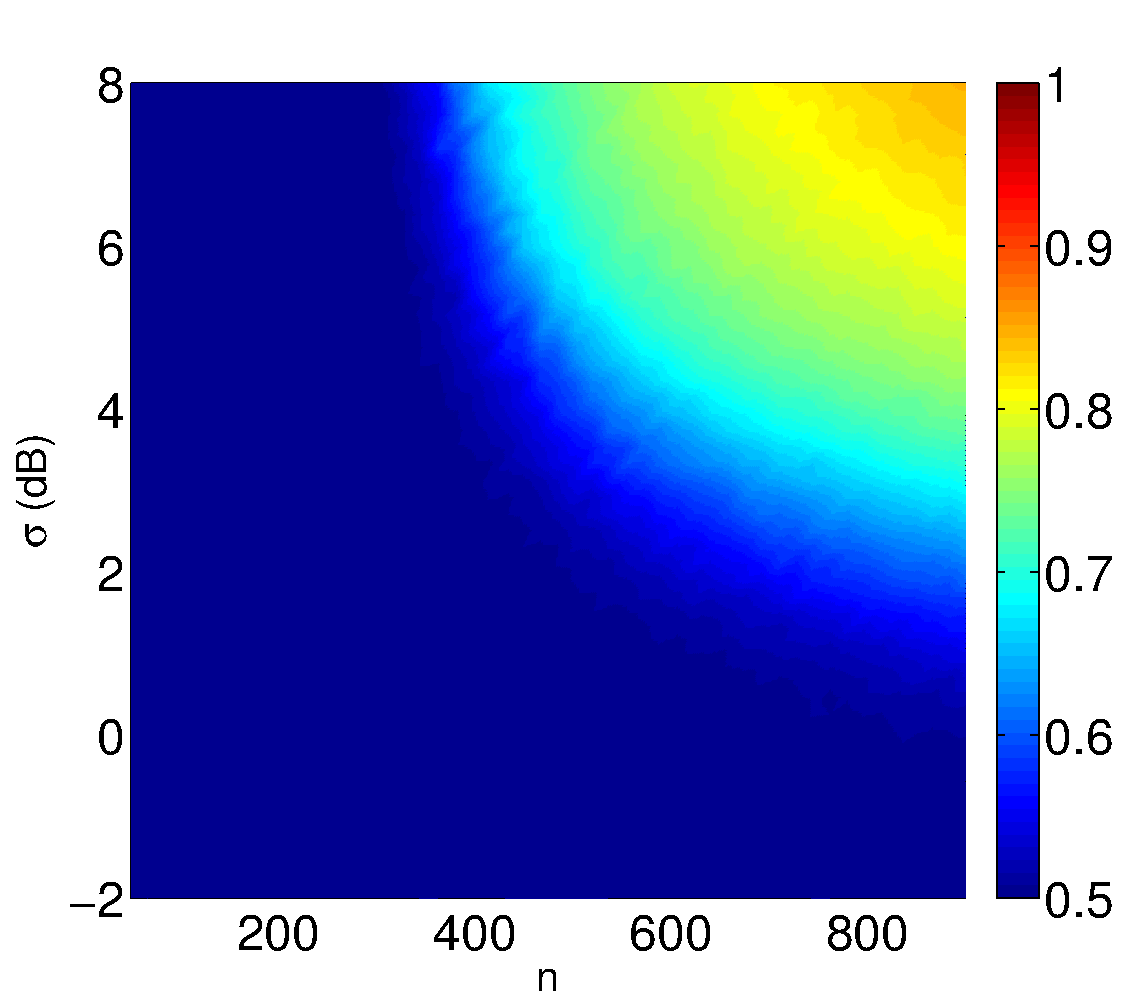
\includegraphics[width=\figwidth]{figures/auc_cca_high_rho.pdf}
    \label{fig:auc_cca_high_rho}
  }
  \caption{AUC results for the plug-in LRT, empirical CCA, and ICCA detectors in
    (\ref{eq:plugin_lrt_stat}), (\ref{eq:cca_plugin_stat}), and
    (\ref{eq:icca_plugin_stat}), respectively. Empirical ROC curves were simulated using
    $2000$ test samples for each hypothesis and averaged over $50$ trials using
    algorithms 2 and 4 of \cite{fawcett2006introduction}. Simulations parameters were
    $d_1=200$, $d_2=150$, and $\rho=0.8$. Each figure plots the AUC for the average ROC curve
    at a different values of SNR, $\sigma=\sigma_1=\sigma_2$, and training samples, $n$.}
  \label{fig:auc_high_rho}
\end{figure}

\begin{figure} 
  \subfigure[Plug-in LRT]{
    \centering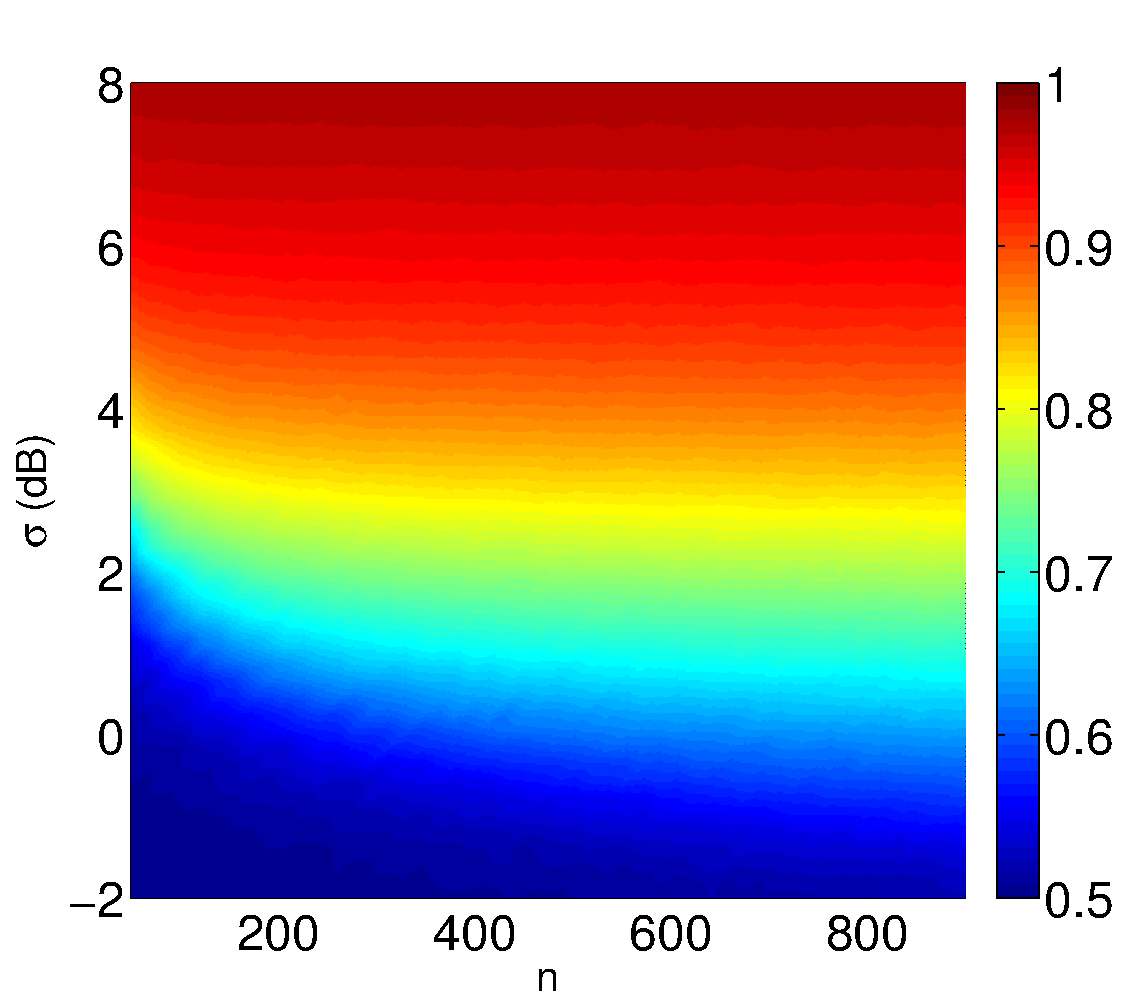
\includegraphics[width=\figwidth]{figures/auc_lrt_low_rho.pdf}
    \label{fig:auc_lrt_low_rho}
  }
  \subfigure[ICCA]{
    \centering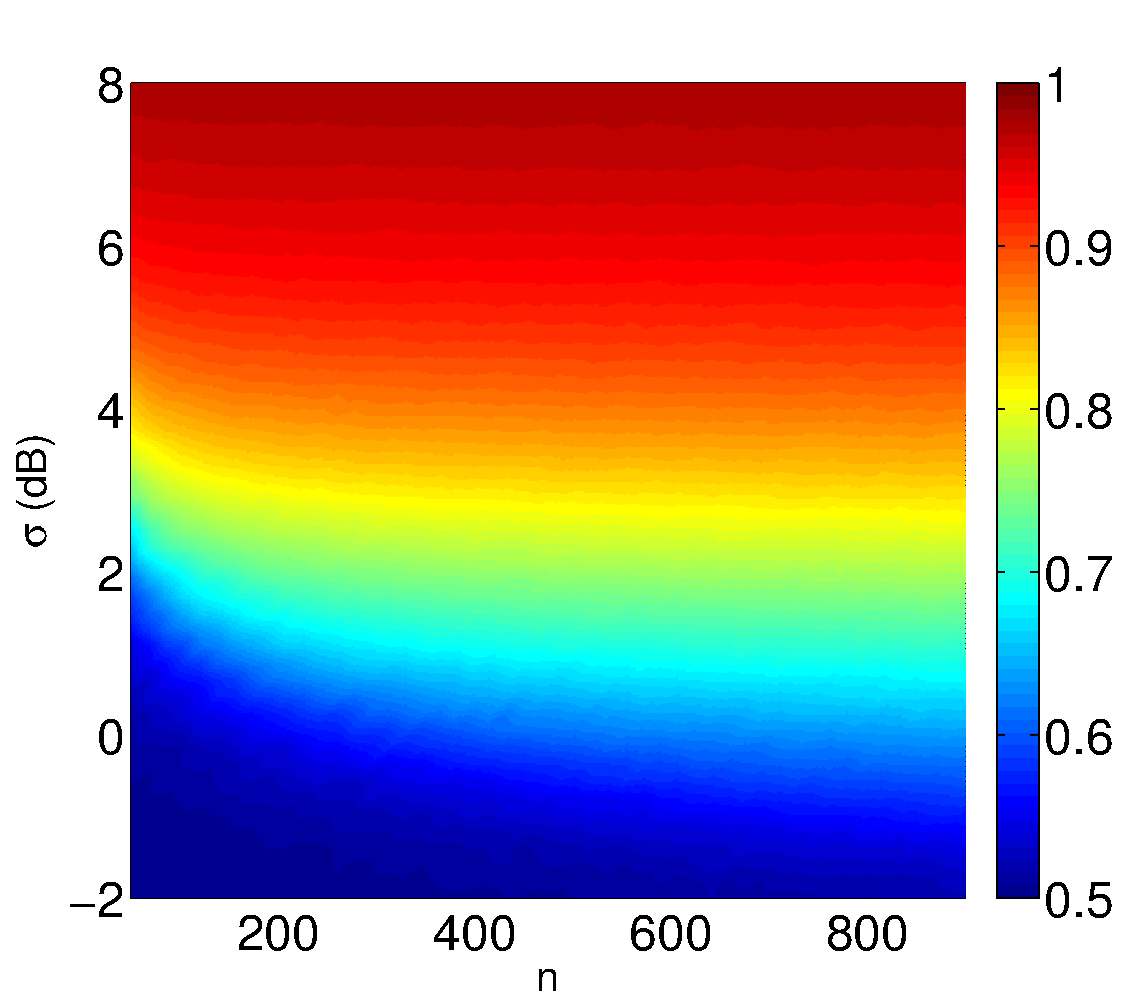
\includegraphics[width=\figwidth]{figures/auc_icca_low_rho.pdf}
    \label{fig:auc_icca_low_rho}
  }
  \subfigure[CCA]{
    \centering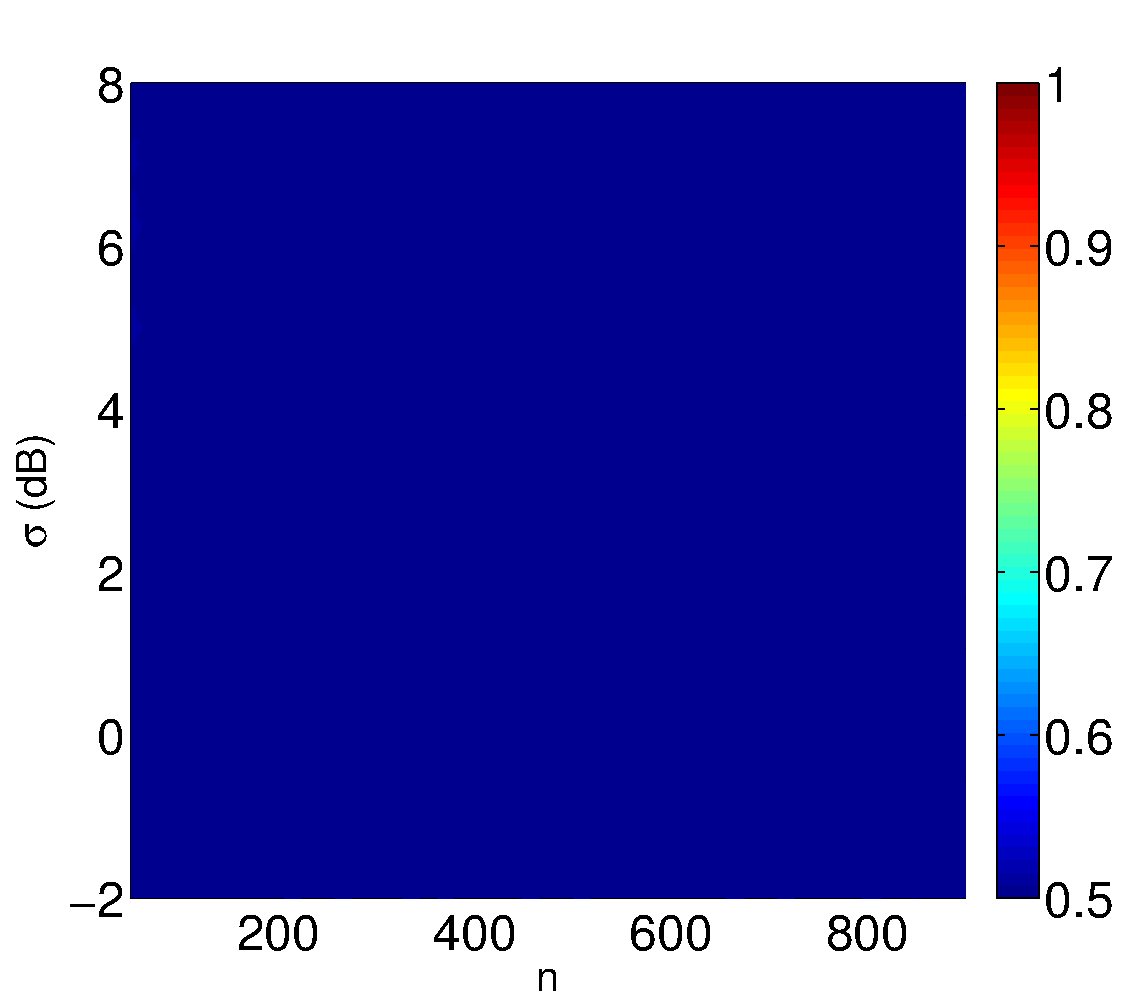
\includegraphics[width=\figwidth]{figures/auc_cca_low_rho.pdf}
    \label{fig:auc_cca_low_rho}
  }
  \caption{AUC results for the plug-in LRT, empirical CCA, and ICCA detectors in
    (\ref{eq:plugin_lrt_stat}), (\ref{eq:cca_plugin_stat}), and
    (\ref{eq:icca_plugin_stat}), respectively. Empirical ROC curves were simulated using
    $2000$ test samples for each hypothesis and averaged over $50$ trials using
    algorithms 2 and 4 of \cite{fawcett2006introduction}. Simulations parameters were
    $d_1=200$, $d_2=150$, and $\rho=0.2$. Each figure plots the AUC for the average ROC curve
    at a different value of SNR, $\sigma=\sigma_1=\sigma_2$, and training samples, $n$.}
  \label{fig:auc_low_rho}
\end{figure}

Evident in both Figures \ref{fig:auc_high_rho} and \ref{fig:auc_low_rho}, the ICCA
detector exhibits the same AUC performance as the plug-in LRT for both values of
$\rho$. This confirms the derivation in the above section. In Figure
\ref{fig:auc_high_rho}, we observe that the CCA detector is extremely suboptimal in the
sample and SNR regime presented. When $n<350=d_1+d_2$, the CCA detector degrades to random
guessing, evident in an AUC of 0.5. The results presented in Chapter
\ref{sec:cca} show that in this sample poor regime, the correlation coefficient
estimate returned by CCA is deterministically 1. It is of no surprise that the subsequent
CCA detector is useless in this regime. Even when $n>d_1+d_2$, the CCA detector achieves a
lower AUC than the ICCA detector. The ICCA detector can tolerate a much lower SNR to achieve
the same AUC performance as the CCA detector.

When decreasing $\rho$ in Figure \ref{fig:auc_low_rho}, the CCA detector observes an even
further performance loss. In the training sample and SNR parameter regime presented,
the CCA detector achieves an AUC of 0.5, indicating it is useless in detection. However,
the plug-in LRT and ICCA detectors show a slight increase in AUC performance. The
intuitive explanation for this result is that decreasing the value of $\rho$ makes the
observations $\yI$ and $\yII$ more independent. Therefore, these observations contain more
information and thus increase detection performance. 

These results are particularly surprising because we began this chapter by deriving the
fact that the LRT detector is equivalent to the CCA detector. However, when using
parameter estimates, the empirical CCA detector no longer is equivalent to the plug-in
detector. As many applications require estimating the covariance matrices used in CCA,
this is an extremely undesirable property of CCA. However, using only the informative
components from our training data, as ICCA does, results in equivalent performance as the
plug-in CCA detector. This performance loss of the empirical CCA detector can be avoided.


%\section*{Performance Loss Heatmaps}

%Defining performance loss for a fixed $P_F$ to be
%\begin{equation}
%  \epsilon = 1 - \frac{P_D^{\text{achieved}}}{P_D^{oracle}}
%\end{equation}

%The following results are for $P_F=0.1$

%\begin{figure} 
%\centering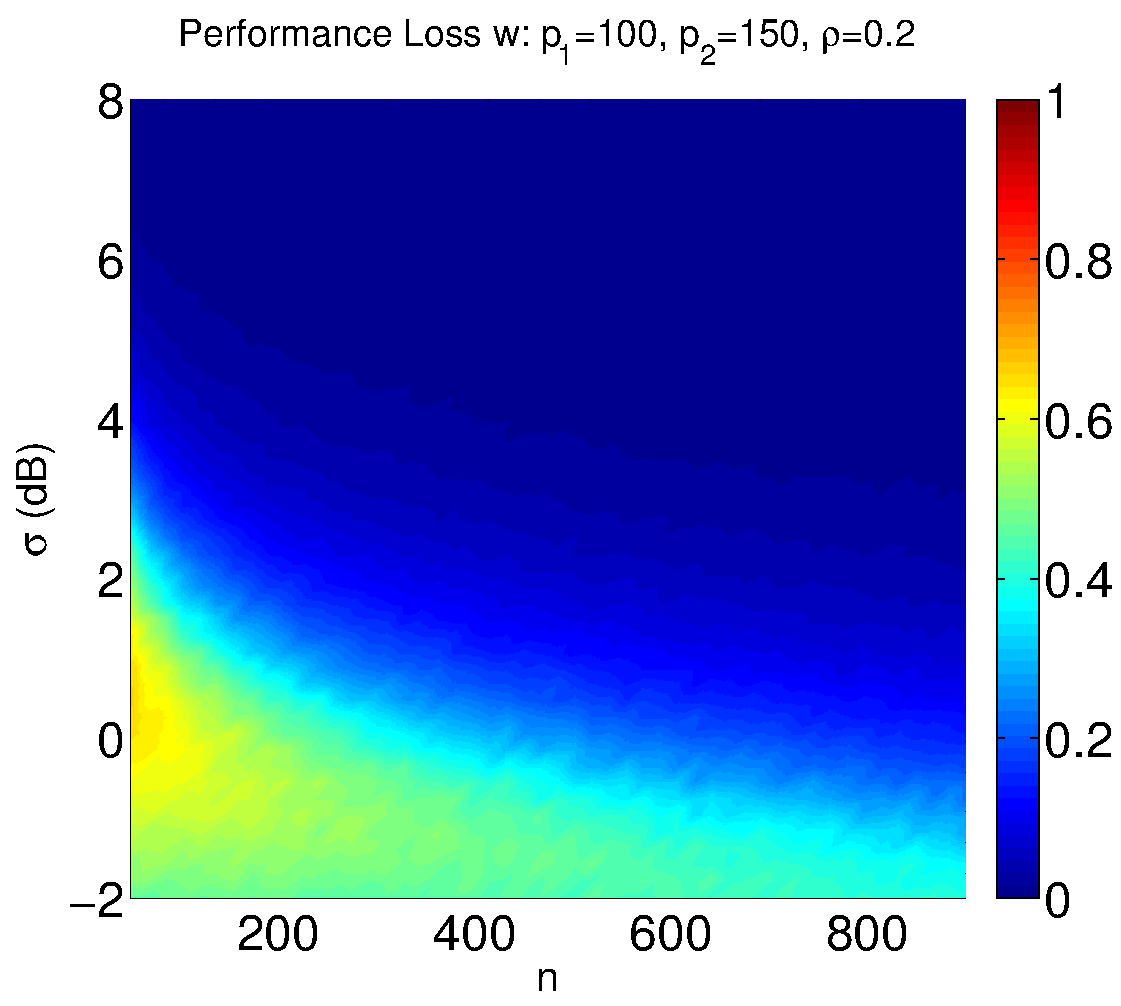
\includegraphics[width=4in]{figures/pl_w_small.pdf}
%\end{figure}

%\begin{figure} 
%\centering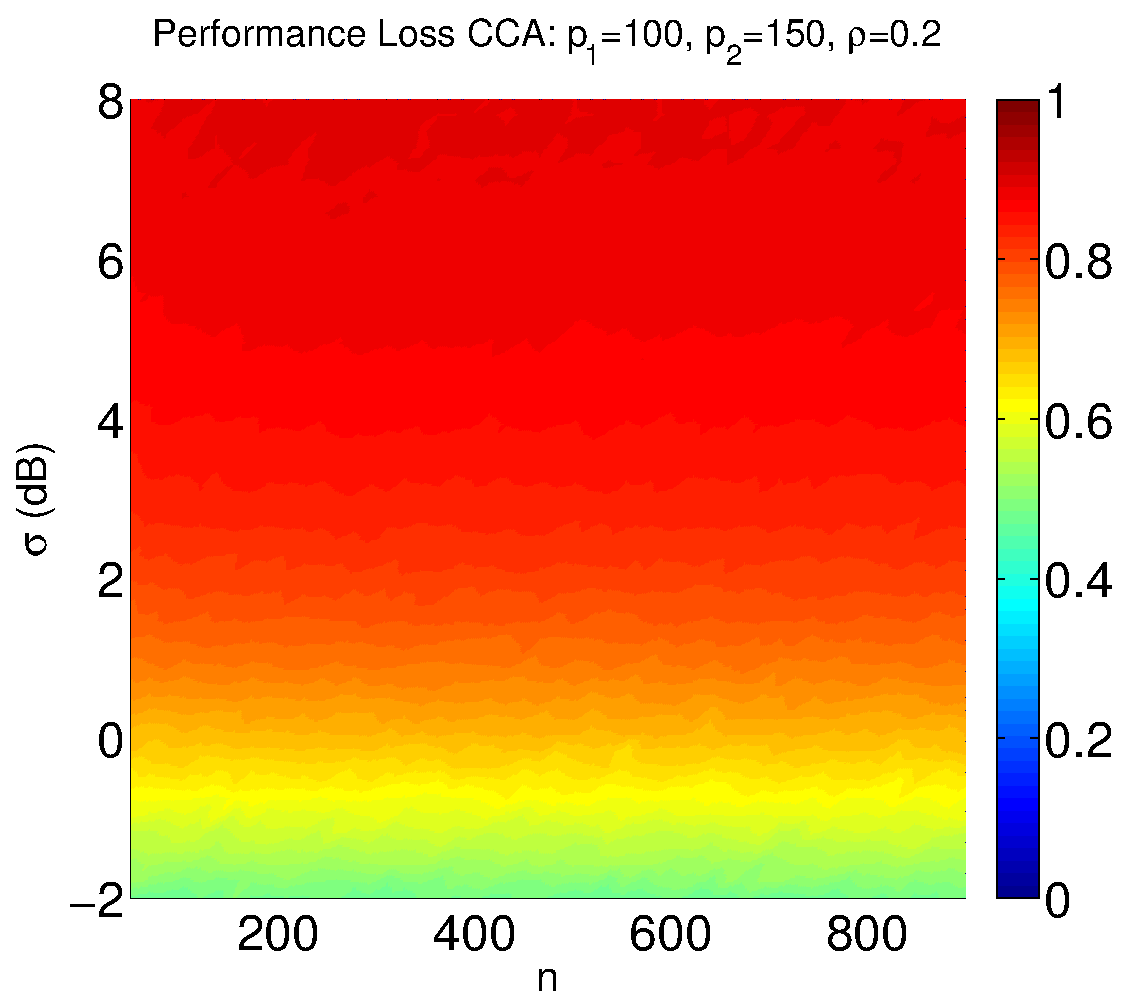
\includegraphics[width=4in]{figures/pl_cca_small.pdf}
%\end{figure}

%\begin{figure} 
%\centering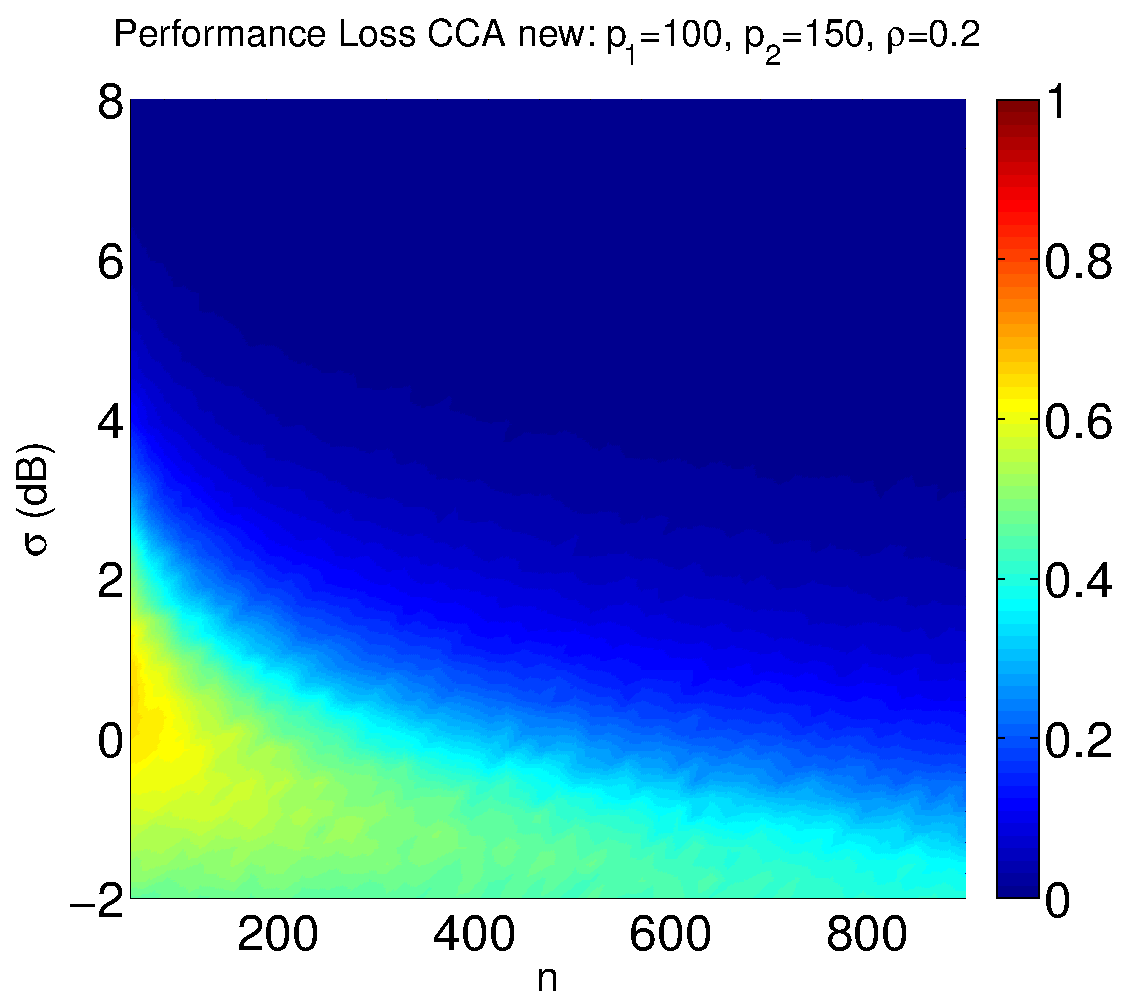
\includegraphics[width=4in]{figures/pl_cca_new_small.pdf}
%\end{figure}


%\begin{figure} 
%\centering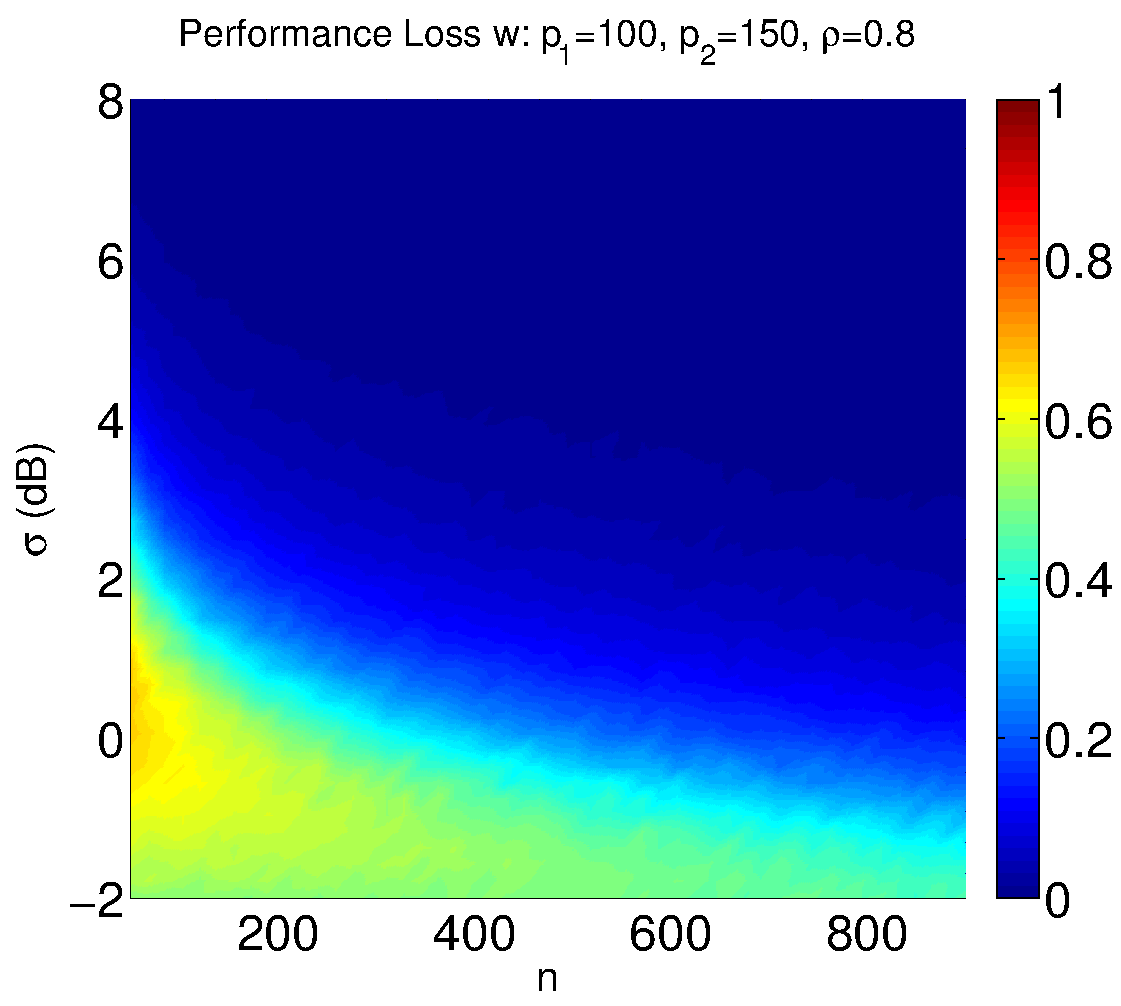
\includegraphics[width=4in]{figures/pl_w_large.pdf}
%\end{figure}

%\begin{figure} 
%\centering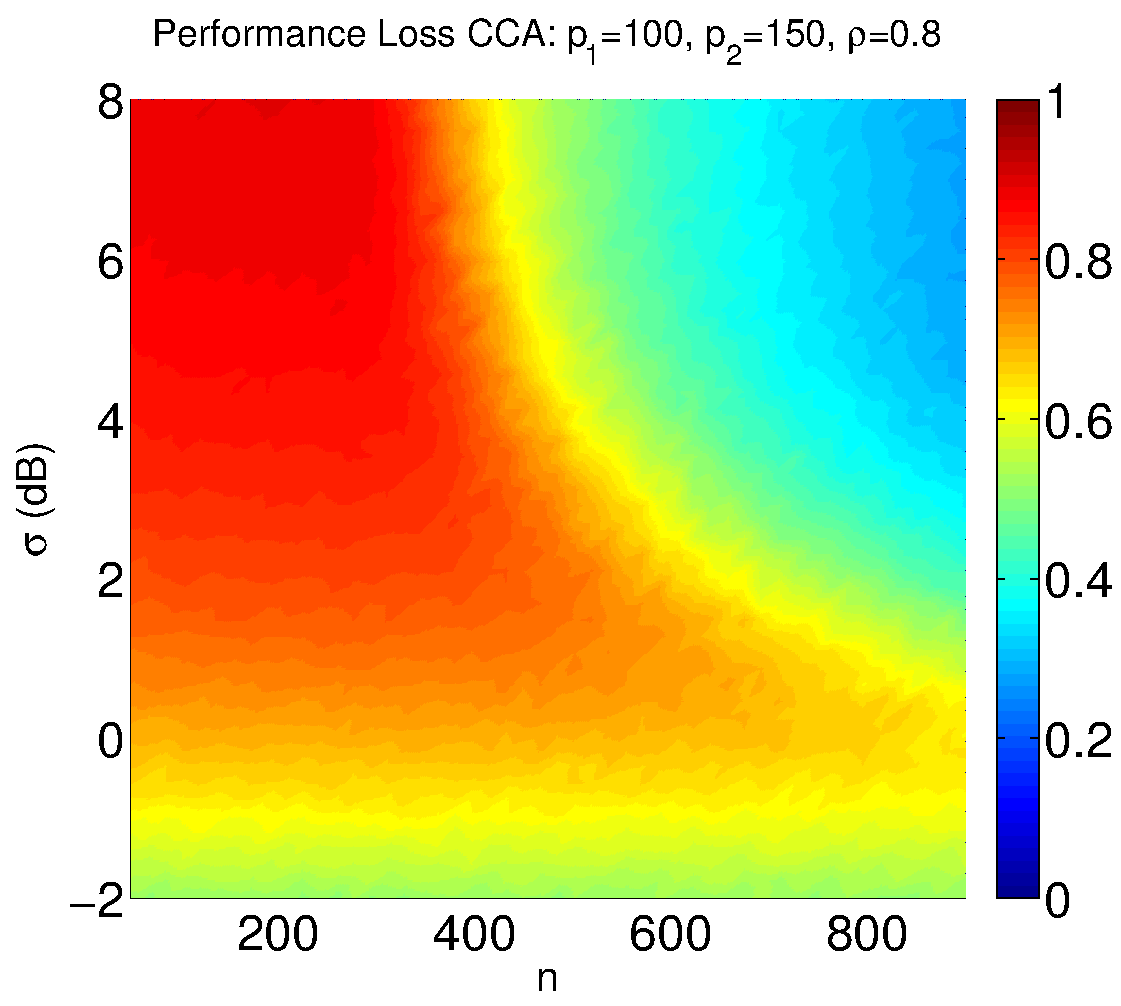
\includegraphics[width=4in]{figures/pl_cca_large.pdf}
%\end{figure}

%\begin{figure} 
%\centering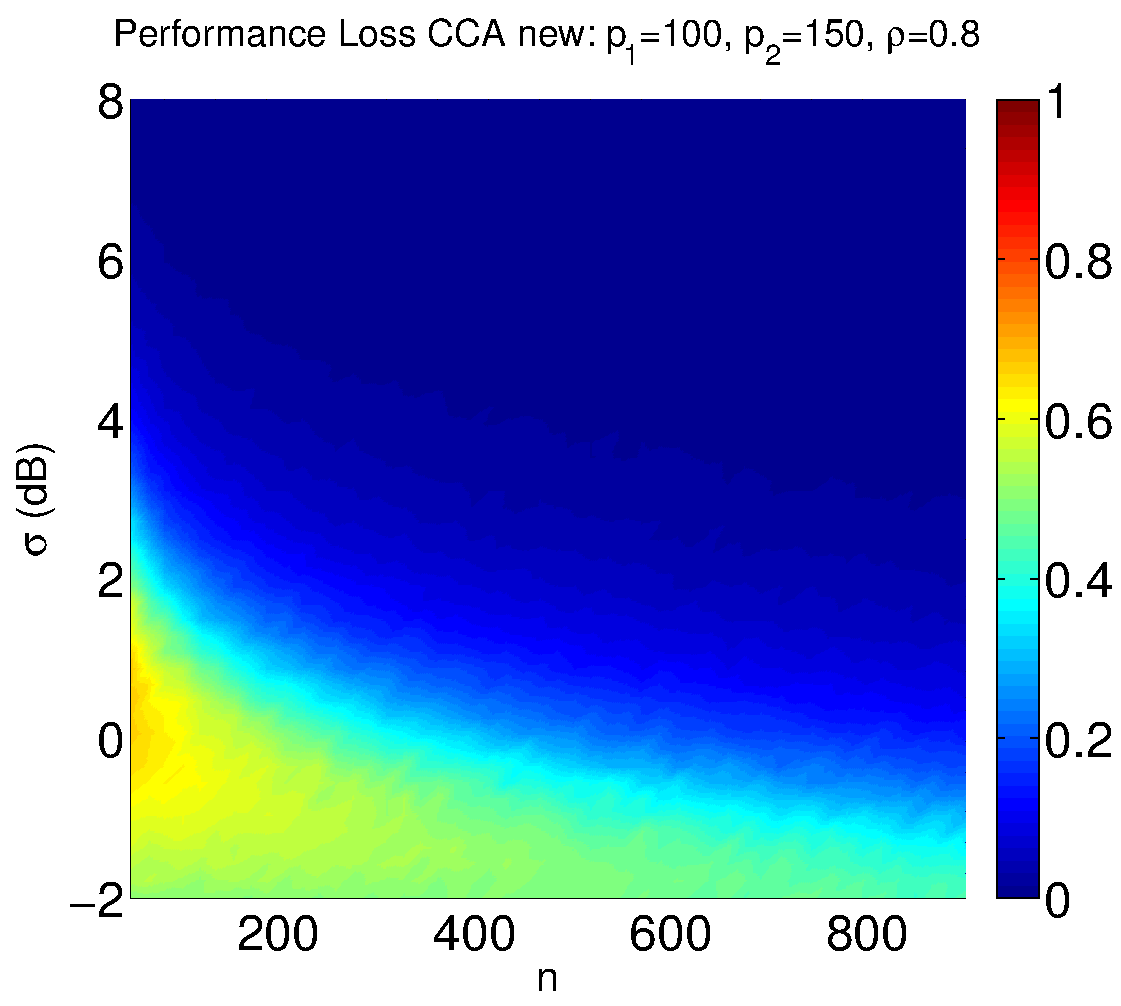
\includegraphics[width=4in]{figures/pl_cca_new_large.pdf}
%\end{figure}
